Se usa ANUGA, versión 4.0.1 \citep{anuga}: volúmenes finitos sobre una malla triangular no estructurada, con el esquema DE1 (Runge--Kutta de segundo orden). Para una mezcla homogénea de densidad constante, ANUGA resuelve la evolución del caudal unitario $\mathbf q=h\mathbf u$ mediante las ecuaciones de conservación de la masa~\eqref{eq:masa} y de la cantidad de movimiento~\eqref{eq:movimiento}:
\begin{align}
\partial_t h+\nabla\cdot\mathbf q&=S_h,\label{eq:masa}\\
\partial_t\mathbf q+\nabla\cdot\left(\frac{\mathbf q\otimes\mathbf q}{h}+\tfrac12 gh^2\mathbf I\right)&=-gh\nabla z-\frac{\boldsymbol\tau_b}{\rho_m}+S_h\mathbf u_\mathrm{in},\label{eq:movimiento}
\end{align}
donde $h$ es el espesor del flujo (\si{m}); $\mathbf u$, la velocidad media en profundidad (\si{m.s^{-1}}); $\mathbf q=h\mathbf u$, el caudal por unidad de ancho (\si{m^2.s^{-1}}); $z$, la elevación del lecho (\si{m}); $g$, la aceleración de gravedad (\si{m.s^{-2}}); $S_h$, la tasa de aporte de espesor (\si{m.s^{-1}}); $\mathbf u_\mathrm{in}$, la velocidad del aporte (\si{m.s^{-1}}); $\boldsymbol\tau_b$, el esfuerzo de corte basal (\si{Pa}); $\rho_m$, la densidad de la mezcla (\si{kg.m^{-3}}); y $\mathbf I$, el tensor identidad. Al dividir por $\rho_m$, constante, no aparece ningún factor de densidad en la presión ni en la gravedad. La resistencia basal es $\boldsymbol\tau_b/\rho_m=ghS_f\,\mathbf u/U$, con $U=|\mathbf u|$ y la pendiente de fricción $S_f$ dada por
\begin{equation}
S_f=\frac{\tau_y}{\rho_m g h}+\frac{K\eta U}{8\rho_m g h^2}+\frac{n_\mathrm{td}^2U^2}{h^{4/3}},\label{eq:friccion}
\end{equation}
donde $\tau_y$ es el esfuerzo de fluencia (\si{Pa}); $\eta$, la viscosidad dinámica de la mezcla (\si{Pa.s}); $K$, el parámetro adimensional de resistencia laminar; y $n_\mathrm{td}$, el coeficiente de Manning equivalente para la turbulencia y la dispersión (\si{s.m^{-1/3}}). El esfuerzo de fluencia y la viscosidad se obtienen de las relaciones reológicas
\begin{equation}
\tau_y=0{,}1\,\alpha_2e^{\beta_2\Cvf},\qquad \eta=0{,}1\,\alpha_1e^{\beta_1\Cvf},\label{eq:reologia}
\end{equation}
donde $\Cvf$ es la concentración volumétrica de la matriz fina; la densidad $\rho_m$ usa, en cambio, la concentración total $\Cvt$ (sección~\ref{sec:marco}). En las simulaciones del barrido se adopta $\Cvt=\Cvf$. Los coeficientes $(\alpha_1,\beta_1,\alpha_2,\beta_2)$ provienen de la tabla~13 de \citet{flo2d2021}, donde $\alpha_1$ se expresa en poises y $\alpha_2$ en \si{dyn.cm^{-2}}; $\beta_1$ y $\beta_2$ son adimensionales. El factor 0,1 de~\eqref{eq:reologia} convierte ambas magnitudes al SI, de modo que $\tau_y$ resulta en \si{Pa} y $\eta$ en \si{Pa.s}. La muestra Glenwood~2 aparece con tres variantes en distintas versiones de la documentación y se trató como sensibilidad. $K$ y $n_\mathrm{td}$ cambian según la superficie: en calles pavimentadas $K=100$ y $n_\mathrm{td}=0{,}025$; en el resto, $K=400$ y $n_\mathrm{td}=0{,}050$.

La resistencia~\eqref{eq:friccion} se aplica como paso fraccionado y se resuelve de forma implícita en cada celda. Con $a=\tau_y/(\rho_m h)$, $b=K\eta/(8\rho_m h^2)$, $c=gn_\mathrm{td}^2/h^{4/3}$ y $r=(U^*-\Delta t\,a)_+$, se obtiene
\begin{equation}
U^{n+1}=\frac{2r}{1+b\Delta t+\sqrt{(1+b\Delta t)^2+4c\Delta t\,r}},\label{eq:resistencia}
\end{equation}
donde el asterisco indica el estado anterior al paso de resistencia; el superíndice $n+1$, el estado posterior a ese paso; $\Delta t$ es el paso temporal y $(x)_+=\max(x,0)$. La solución~\eqref{eq:resistencia} cumple $0\le U^{n+1}\le U^*$, conserva la dirección, disipa energía y no modifica $h$. Si $|\mathbf q^*|\le\Delta t\,\tau_y/\rho_m$, la celda se detiene y puede reactivarse en pasos posteriores. La fricción de Manning propia de ANUGA se anula para no duplicar la resistencia.

La mezcla entra mediante un hidrograma triangular de caudal pico $Q_p$, volumen de mezcla $V_m$ y tiempo al pico de \SI{600}{s}, con base $T_B=2V_m/Q_p$. Cada fuente agrega en un círculo de \SI{14}{m} de radio el incremento de espesor $\Delta h$ correspondiente al volumen aportado por el hidrograma durante el paso, junto con su momento: $h^+=h^-+\Delta h$ y $\mathbf q^+=\mathbf q^-+\Delta h\,\mathbf u_\mathrm{in}$, donde los superíndices $-$ y $+$ indican los estados anterior y posterior al aporte, y $\mathbf u_\mathrm{in}$ se orienta según el eje del cauce. Cuando $Q=0$ no hay forzamiento. En H3, cada fuente recibe la fracción del hidrograma correspondiente al área de su cuenca. La malla de la primera generación tiene unos \num{4,3e5} triángulos: \SI{40}{m^2} en el corredor entre los cauces y Padre Hurtado (lado equivalente de unos \SI{10}{m}) y \SI{600}{m^2} fuera de él. La aceleración de gravedad es $g=\SI{9,8}{m.s^{-2}}$ en todo el modelo. En la primera generación, las simulaciones duran $T_B+\SI{1200}{s}$ y en cada una se registra el balance de volumen. Las variantes de ciudad, lluvia medida y malla fina del campus se describen en las secciones~\ref{sec:res-v4} y~\ref{sec:res-posterior}.

\begin{table}[htbp]\centering\small
\caption{Parámetros físicos y numéricos aplicados en las simulaciones. Los coeficientes reológicos son los de la tabla de muestras de O'Brien y Julien recopilada en el manual de FLO-2D \citep{flo2d2021}; $\tau_y=0{,}1\,\alpha_2e^{\beta_2C_v}$ en Pa y $\eta=0{,}1\,\alpha_1e^{\beta_1C_v}$ en Pa\,s.}\label{tab:parametros}
\begin{adjustbox}{max width=\textwidth}\begin{tabular}{lrrrrrrr}\toprule
Muestra & $\alpha_1$ & $\beta_1$ & $\alpha_2$ & $\beta_2$ & \multicolumn{3}{c}{$\tau_y$ (Pa) / $\eta$ (Pa\,s) con $C_v=$}\\\cmidrule(l){6-8}
 & & & & & 0,35 & 0,40 & 0,45\\\midrule
Glenwood 1 & 0{,}0028 & 23{,}00 & 0{,}0345 & 20{,}10 & 3{,}9 / 0{,}89 & 10{,}7 / 2{,}80 & 29{,}2 / 8{,}85\\
Glenwood 2a & 0{,}0648 & 6{,}20 & 0{,}0765 & 16{,}90 & 2{,}8 / 0{,}06 & 6{,}6 / 0{,}08 & 15{,}4 / 0{,}11\\
Glenwood 2b & 0{,}6480 & 6{,}20 & 0{,}0765 & 16{,}90 & 2{,}8 / 0{,}57 & 6{,}6 / 0{,}77 & 15{,}4 / 1{,}06\\
Glenwood 2c & 0{,}6480 & 8{,}20 & 0{,}0765 & 16{,}90 & 2{,}8 / 1{,}14 & 6{,}6 / 1{,}72 & 15{,}4 / 2{,}59\\
Aspen 1 & 0{,}0360 & 22{,}10 & 0{,}1810 & 25{,}70 & 145{,}9 / 8{,}23 & 527{,}5 / 24{,}86 & 1906{,}8 / 75{,}05\\
Aspen 2 & 0{,}0538 & 14{,}50 & 2{,}7200 & 10{,}40 & 10{,}4 / 0{,}86 & 17{,}4 / 1{,}78 & 29{,}3 / 3{,}67\\
\midrule
\multicolumn{8}{l}{\textbf{Mezcla y constantes}}\\
\multicolumn{5}{l}{Densidad del agua $\rho_w$ / de los sólidos $\rho_s$} & \multicolumn{3}{r}{\SI{1000}{kg/m^3} / \SI{2650}{kg/m^3}}\\
\multicolumn{5}{l}{Densidad de la mezcla $\rho_m=\rho_w+C_v(\rho_s-\rho_w)$, $C_v=0{,}35/0{,}40/0{,}45$} & \multicolumn{3}{r}{1578 / 1660 / 1742 kg/m$^3$}\\
\multicolumn{5}{l}{Gravedad $g$} & \multicolumn{3}{r}{\SI{9,8}{m/s^2}}\\
\multicolumn{5}{l}{Resistencia laminar $K$ (calles / resto)} & \multicolumn{3}{r}{100 / 400}\\
\multicolumn{5}{l}{Manning turbulento-dispersivo $n_{td}$ (calles / resto)} & \multicolumn{3}{r}{0,025 / 0,050 s\,m$^{-1/3}$}\\
\multicolumn{8}{l}{\textbf{Entrada, malla y cálculo}}\\
\multicolumn{5}{l}{Volumen de mezcla $V$ / caudal pico $Q_p$ / tiempo al pico $t_p$} & \multicolumn{3}{r}{80--300 mil m$^3$ / 100--250 m$^3$/s / 600 s}\\
\multicolumn{5}{l}{Velocidad de entrada / radio de cada fuente} & \multicolumn{3}{r}{2 m/s / 14 m}\\
\multicolumn{5}{l}{Área máxima de triángulo (corredor / resto); triángulos, primera generación} & \multicolumn{3}{r}{40 / 600 m$^2$; $\approx$430\,000}\\
\multicolumn{5}{l}{Grilla del terreno; rebaje de calles; altura supuesta de edificios} & \multicolumn{3}{r}{4 m; 0,15 m; 6 m}\\
\multicolumn{5}{l}{Número de Courant (cribado / lluvia / final)} & \multicolumn{3}{r}{1 / 0,5 / $\le$0,25}\\
\multicolumn{5}{l}{Umbral de mojado para la evaluación $h^*$} & \multicolumn{3}{r}{5 cm (sensibilidad 2 y 10 cm)}\\
\bottomrule\end{tabular}\end{adjustbox}\end{table}

\begin{figure}[htbp]\centering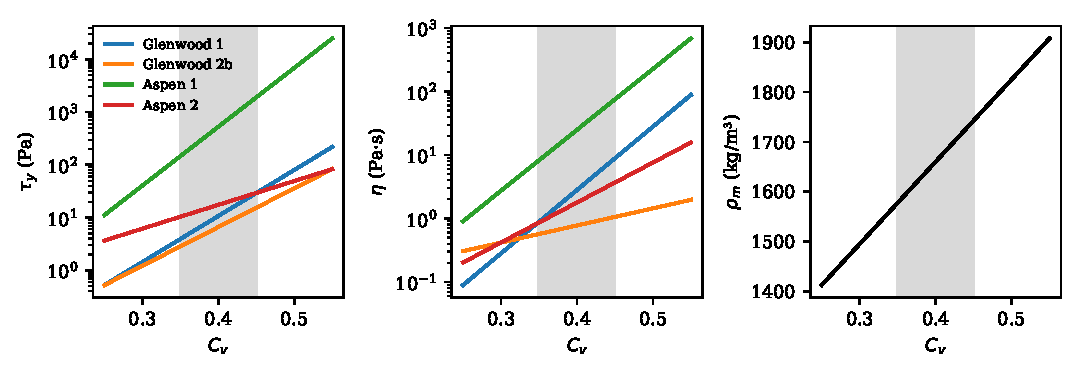
\includegraphics[width=\textwidth]{reologia}\caption{Propiedades calculadas de la mezcla según la concentración volumétrica de sólidos $C_v$ para las muestras ensayadas: esfuerzo de fluencia $\tau_y$, viscosidad $\eta$ y densidad $\rho_m$. La franja gris indica el rango inicial (0,35--0,45); los ensayos posteriores amplían las concentraciones (sección~\ref{sec:res-posterior}).}\label{fig:reologia}\end{figure}
